\documentclass[a4paper, 12pt]{report}
\usepackage{graphicx}
\usepackage{xspace}
\usepackage[margin= 1in,includefoot]{geometry}
\newcommand\nth{\textsuperscript{th}\xspace}
\usepackage{xcolor}
\usepackage{lipsum}
\usepackage{listings}
\begin{document}
\begin{figure}

\includegraphics[scale=.63]{medipol.png}
\centering
\end{figure}
\begin{titlepage}
\title{Fall 2021, Computer Vision \\ Homework 2}
\author{by 64160010 - Rumeysa ÇELİK}
\maketitle
\end{titlepage}
\section*{{\textbf{Problem Set 2}}}
\textbf{Problem 1:}
Design and implement Hough Transform method for finding lines. 
\\ \\
You can use OpenCV functions to find edges, such as Canny operator, but you may not use any Hough Transform functions. Convert a color image to grayscale before applying an edge detector.
\\ \\
Specifically, create a Hough transform class including the following functions:
\begin{itemize}
\item hough$\_$lines$\_$acc: Takes an edge image as input, and two optional parameters Theta Resolution and Rho Resolution, which indicates the cell size for theta and rho parameters.Returns an accumulator matrix H, and cell locations theta and rho. 
\item hough$\_$peaks:Returns the peak locations (theta and rho) for a given H, theta, and rho arrays. The function also should take a threshold value t to eliminate weak peaks that are less than t, and another parameter s to return the strongest s peaks.
\item hough$\_$lines$\_$draw: Draw color lines corresponding to the peaks found.
\end{itemize}
Finally, write a script file to get the results on some input images.Compare your results with the results obtained using OpenCV Hough transform. 
\\ \\
{\color{blue}{OpenCV functions were used to find edges like the Canny operator, but no Hough Transform functions were used. \\ Specifically, a Hough transform class was created that includes "hough$\_$lines$\_$acc, hough$\_$peaks and hough$\_$lines$\_$draw".
\\ \\  \\ \\ \\
\textbf{INPUT IMAGE:}
\\
\begin{figure}[h]
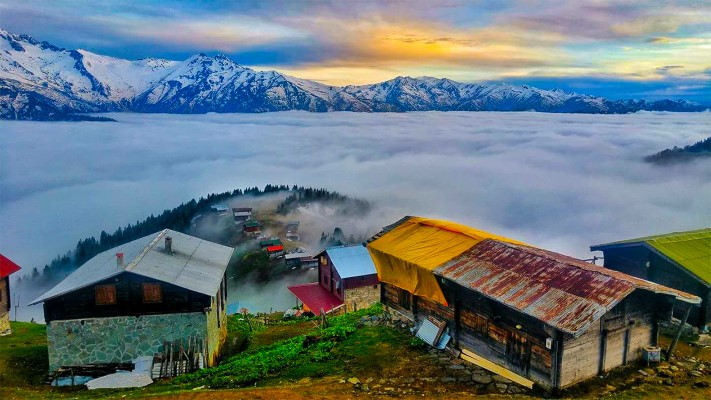
\includegraphics[scale=1.23]{pokut.jpeg}
\centering
\end{figure}
\newpage
\textbf{Code:}

\definecolor{codegreen}{rgb}{0,0.6,0}
\definecolor{codegray}{rgb}{0.5,0.5,0.5}
\definecolor{codepurple}{rgb}{0.58,0,0.82}
\definecolor{backcolour}{rgb}{0.95,0.95,0.92}

\lstdefinestyle{mystyle}{
    backgroundcolor=\color{backcolour},   
    commentstyle=\color{codegreen},
    keywordstyle=\color{magenta},
    numberstyle=\tiny\color{codegray},
    stringstyle=\color{codepurple},
    basicstyle=\ttfamily\footnotesize,
    breakatwhitespace=false,         
    breaklines=true,                 
    captionpos=b,                    
    keepspaces=true,                 
    numbers=left,                    
    numbersep=5pt,                  
    showspaces=false,                
    showstringspaces=false,
    showtabs=false,                  
    tabsize=2
}

\lstset{style=mystyle}
\begin{lstlisting}[language=Python]

# -*- coding: utf-8 -*-
"""
Created on Fri Nov 12 19:11:12 2021

@author: Rumeysa CELIK
"""

import numpy as np
import cv2

#hough_lines_acc:Takes an edge image as input, and two optionalparameters ThetaResolutionand RhoResolution, which indicates the cell size for theta and rho parameters.Returns an accumulator matrix H, and cell locations thetaand rho.

#hough_peaks:Returns the peak locations (theta and rho) for a given H, theta, and rhoarrays. The function also should take a threshold value tto eliminate weak peaks that are less than t, and another parameter sto return the strongest s peaks.

#hough_lines_draw:Draw color lines corresponding to the peaks found.

image = cv2.imread('input/pokut.jpeg')
RGB_img = cv2.cvtColor(image, cv2.COLOR_BGR2RGB)
imageGray = cv2.cvtColor(RGB_img, cv2.COLOR_RGB2GRAY)
imageBlur = cv2.GaussianBlur(imageGray, (5, 5), 1.5)
canny_edges = cv2.Canny(imageBlur, 50, 50)


def generateHoughLines(img, indices, rhos, thetas):
    for i in range(len(indices)):
        rho = rhos[indices[i][0]]
        theta = thetas[indices[i][1]]
        a = np.cos(theta)
        b = np.sin(theta)
        x0 = a * rho
        y0 = b * rho
        x1 = int(x0 + 1000 * -b)
        y1 = int(y0 + 1000 * a)
        x2 = int(x0 - 1000 * -b)
        y2 = int(y0 - 1000 * a)
        cv2.line(img, (x1, y1), (x2, y2), (255, 0, 0), 2)


def houghLocations(H, num_peaks):
    size = 3
    indices = []
    a = np.copy(H)
    for i in range(num_peaks):
        idx = np.argmax(a)
        AIdx = np.unravel_index(idx, a.shape)
        indices.append(AIdx)

        idx_y, idx_x = AIdx
        if (idx_x - (size / 2)) < 0:
            min_x = 0
        else:
            min_x = idx_x - (size / 2)
        if (idx_x + (size / 2) + 1) > H.shape[1]:
            max_x = H.shape[1]
        else:
            max_x = idx_x + (size / 2) + 1

        if (idx_y - (size / 2)) < 0:
            min_y = 0
        else:
            min_y = idx_y - (size / 2)
        if (idx_y + (size / 2) + 1) > H.shape[0]:
            max_y = H.shape[0]
        else:
            max_y = idx_y + (size / 2) + 1

        for x in range(int(min_x), int(max_x)):
            for y in range(int(min_y), int(max_y)):
                a[y, x] = 0
                if x == min_x or x == (max_x - 1):
                    H[y, x] = 255
                if y == min_y or y == (max_y - 1):
                    H[y, x] = 255
    return indices, H


def hough(img, rho_resolution=1, theta_resolution=1):
    height, width = img.shape
    img_diagonal = np.ceil(np.sqrt(height ** 2 + width ** 2))
    rhos = np.arange(-img_diagonal, img_diagonal + 1, rho_resolution)
    thetas = np.deg2rad(np.arange(-90, 90, theta_resolution))

    H = np.zeros((len(rhos), len(thetas)), dtype=np.uint64)
    y_idxs, x_idxs = np.nonzero(img)
    for i in range(len(x_idxs)):
        x = x_idxs[i]
        y = y_idxs[i]
        for j in range(len(thetas)):
            rho = int((x * np.cos(thetas[j]) +
                       y * np.sin(thetas[j])) + img_diagonal)
            H[rho, j] += 1
    return H, rhos, thetas


if __name__ == "__main__":
    H, rhos, thetas = hough(canny_edges)
    indices, H = houghLocations(H, 25)

    generateHoughLines(image, indices, rhos, thetas)

    cv2.imshow('Image with Lines', image)
    cv2.imwrite('output.jpeg', image)
    cv2.waitKey(0)


\end{lstlisting}
\textbf{OUTPUT:}

\begin{figure}[h]
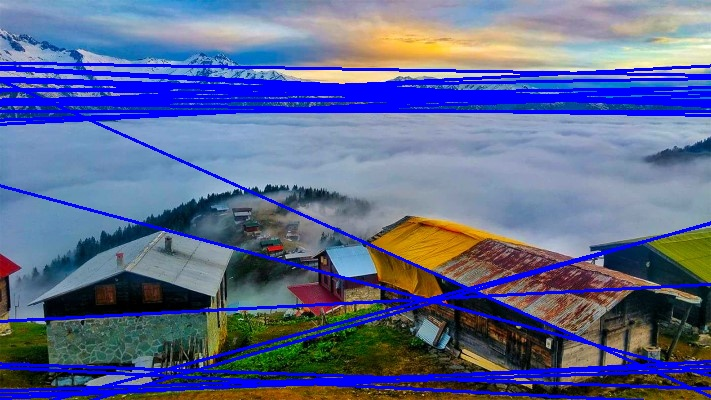
\includegraphics[scale=.33]{output.jpeg}
\centering
\end{figure}


\setlength{\parindent}{0pt}{\textbf{Problem 2:} Write a script file to demonstrate your Hough based line detector on live video.}
\\ \\
A script was written to show the Hough-based line detector in live video.
\\ \\
\textbf{Code:}

\definecolor{codegreen}{rgb}{0,0.6,0}
\definecolor{codegray}{rgb}{0.5,0.5,0.5}
\definecolor{codepurple}{rgb}{0.58,0,0.82}
\definecolor{backcolour}{rgb}{0.95,0.95,0.92}

\lstdefinestyle{mystyle}{
    backgroundcolor=\color{backcolour},   
    commentstyle=\color{codegreen},
    keywordstyle=\color{magenta},
    numberstyle=\tiny\color{codegray},
    stringstyle=\color{codepurple},
    basicstyle=\ttfamily\footnotesize,
    breakatwhitespace=false,         
    breaklines=true,                 
    captionpos=b,                    
    keepspaces=true,                 
    numbers=left,                    
    numbersep=5pt,                  
    showspaces=false,                
    showstringspaces=false,
    showtabs=false,                  
    tabsize=2
}

\lstset{style=mystyle}
\begin{lstlisting}[language=Python]

# -*- coding: utf-8 -*-
"""
Created on Sun Nov 14 23:11:12 2021

@author: Rumeysa CELIK
"""

import numpy as np
import cv2

#Write a script file to demonstrate your Hough based line detector on live video.

def generateHoughLines(img, indices, rhos, thetas):
    for i in range(len(indices)):
        rho = rhos[indices[i][0]]
        theta = thetas[indices[i][1]]
        a = np.cos(theta)
        b = np.sin(theta)
        x0 = a * rho
        y0 = b * rho
        x1 = int(x0 + 1000 * -b)
        y1 = int(y0 + 1000 * a)
        x2 = int(x0 - 1000 * -b)
        y2 = int(y0 - 1000 * a)
        cv2.line(img, (x1, y1), (x2, y2), (255, 0, 0), 2)


def hough(img, rho_resolution=1, theta_resolution=1):
    height, width = img.shape
    img_diagonal = np.ceil(np.sqrt(height ** 2 + width ** 2))
    rhos = np.arange(-img_diagonal, img_diagonal + 1, rho_resolution)
    thetas = np.deg2rad(np.arange(-90, 90, theta_resolution))

    H = np.zeros((len(rhos), len(thetas)), dtype=np.uint64)
    y_idxs, x_idxs = np.nonzero(img)
    for i in range(len(x_idxs)):
        x = x_idxs[i]
        y = y_idxs[i]
        for j in range(len(thetas)):
            rho = int((x * np.cos(thetas[j]) +
                       y * np.sin(thetas[j])) + img_diagonal)
            H[rho, j] += 1
    return H, rhos, thetas


def houghLocations(H, num_peaks):
    indices = []
    size = 10
    a = np.copy(H)
    for i in range(num_peaks):
        idx = np.argmax(a)
        AInd = np.unravel_index(idx, a.shape)
        indices.append(AInd)

        idx_y, idx_x = AInd
        if (idx_x - (size / 2)) < 0:
            min_x = 0
        else:
            min_x = idx_x - (size / 2)
        if (idx_x + (size / 2) + 1) > H.shape[1]:
            max_x = H.shape[1]
        else:
            max_x = idx_x + (size / 2) + 1

        if (idx_y - (size / 2)) < 0:
            min_y = 0
        else:
            min_y = idx_y - (size / 2)
        if (idx_y + (size / 2) + 1) > H.shape[0]:
            max_y = H.shape[0]
        else:
            max_y = idx_y + (size / 2) + 1

        for x in range(int(min_x), int(max_x)):
            for y in range(int(min_y), int(max_y)):
                a[y, x] = 0
                if x == min_x or x == (max_x - 1):
                    H[y, x] = 255
                if y == min_y or y == (max_y - 1):
                    H[y, x] = 255
    return indices, H


if __name__ == "__main__":
    video = cv2.VideoCapture(0)
    a = 0
    while True:
        a = a + 1
        check, frame = video.read()
        gray = cv2.cvtColor(frame, cv2.COLOR_BGR2GRAY)
        edges = cv2.Canny(frame, 100, 200)
        H, rhos, thetas = hough(edges)
        indices, H = houghLocations(H, 10)
        generateHoughLines(frame, indices, rhos, thetas)
        cv2.imshow("Captured Video", frame)
        cv2.imwrite('VideOutput.jpg', frame)
        key = cv2.waitKey(1)
        if key == ord('w'):
            break

    video.release()



\end{lstlisting}
\textbf{OUTPUT:}

\begin{figure}[h]
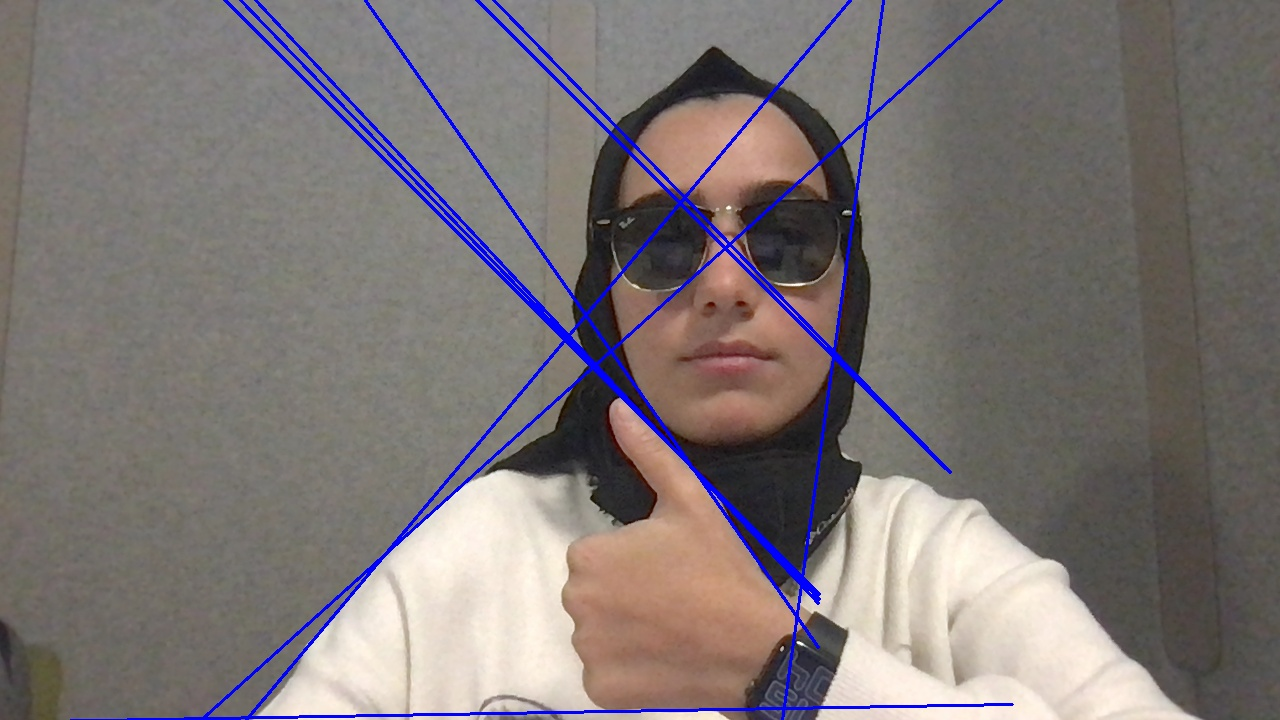
\includegraphics[scale=.27]{VideOutput.jpg}
\centering
\end{figure}




}}

































\end{document}